\section{DESENVOLVIMENTO}

\subsection{FORMATAÇÃO DOS TÍTULOS}

\begin{itemize} 
    \item Título primário: Caixa alta e negritoç
    \item Título secundário: Caixa alta;
    \item Título terciário: Negrito;
    \item Título quaternário: ''Normal'';
    \item Título sem indicativos numéricos: Caixa alta, negrito, centralizado;
\end{itemize}

Títulos que ocupem mais de uma linha devem ser, a partir da segunda linha, alinhados abaixo da primeira letra da primeira palavra do título.

\subsubsection{Exemplo de titulo terciário}

\lipsum[2]

\subsection{REGRAS PARA O SUMÁRIO}

\begin{figure}[h]
    \centering
    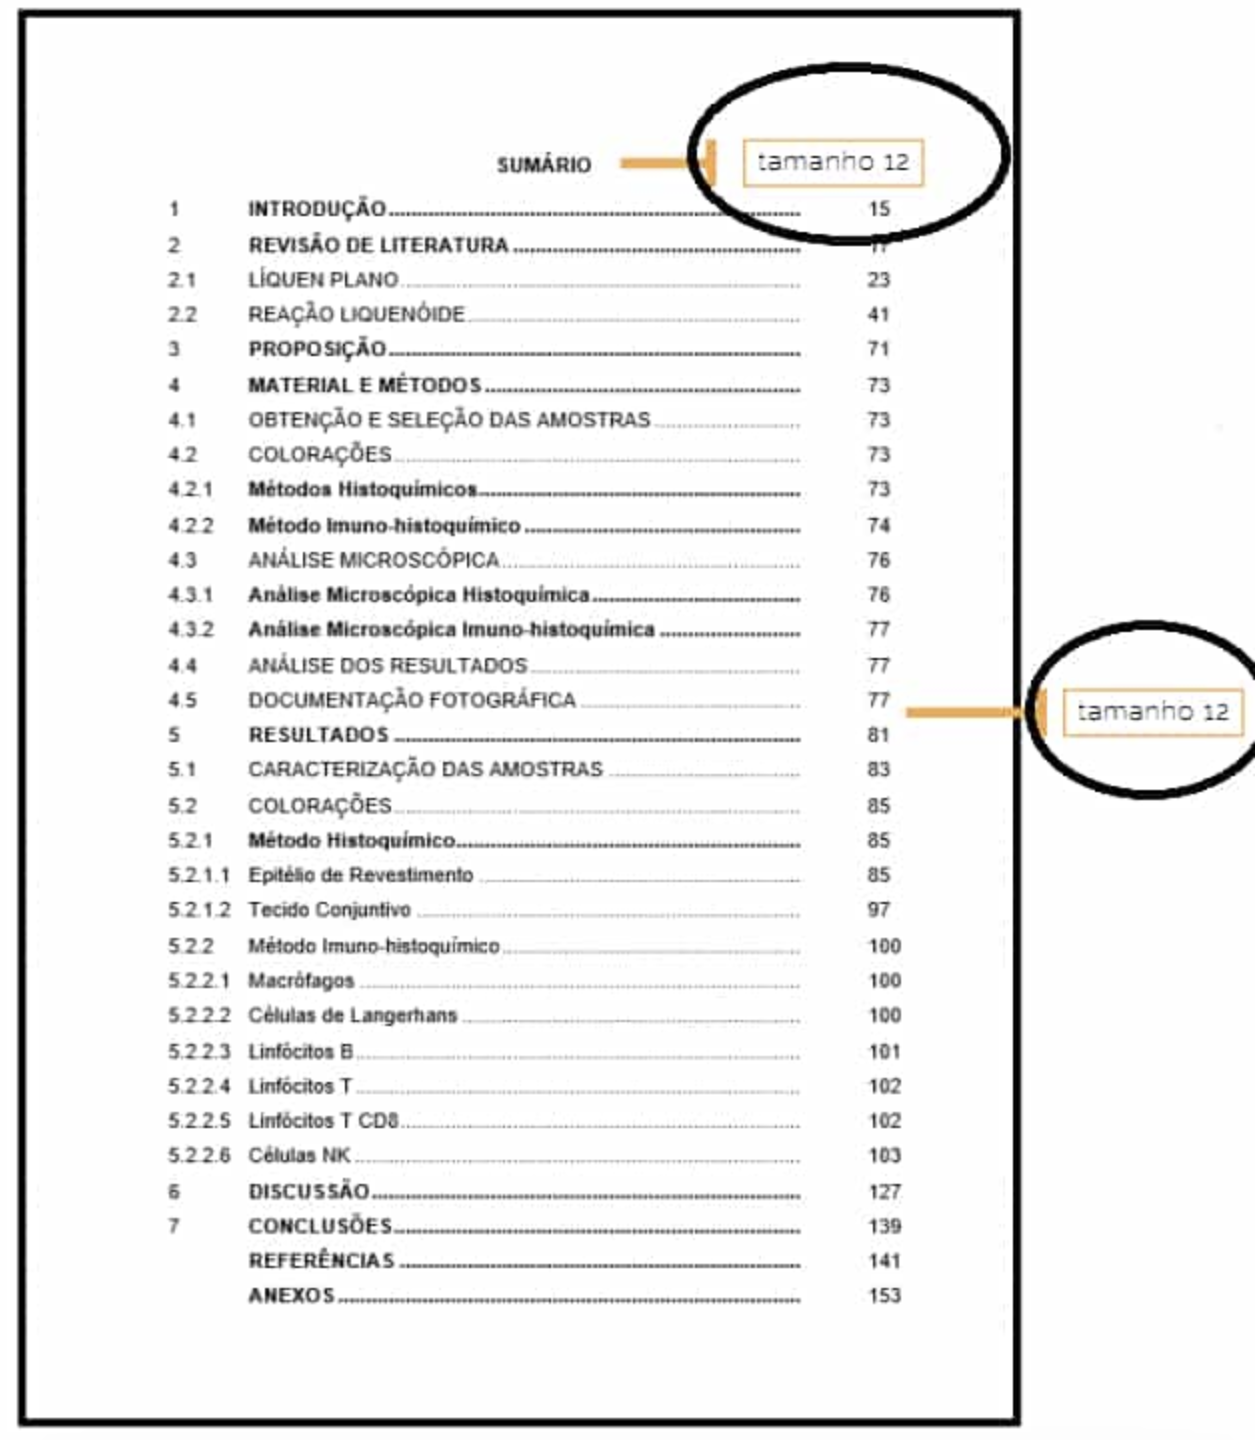
\includegraphics[width=0.9\textwidth]{Figuras/exemplo_sumario.png} % Change to the path of your image
    \caption{Exemplo de um sumário.}
    \label{fig:exemplo_sumario}
\end{figure}

\begin{itemize}
    \item A margem superior e esquerda deverá ser de 3 cm;
    \item A margem inferior e direita deverá ser de 2 cm;
    \item O título deverá ficar centralizado e em letra maiúscula;
    \item O sumário deverá ficar antes da introdução;
    \item Você deverá organizar de acordo com os capítulos, seções e partes, tudo na ordem que seu trabalho será!
    \item O sumário deverá ficar depois da capa, folha de rosto, folha de aprovação, dedicatória, resumo ou listas;
    \item A palavra “sumário” ficará no topo da página em negrito, com a mesma fonte e tamanho do resto do texto;
    \item O espaçamento entre as linhas deverá ser de 1,5;
    \item O tamanho da fonte deverá ser 12;
    \item Não deverão conter outros textos, apenas os títulos das divisões e subdivisões;
    \item Os capítulos devem ser escritos com todas as letras em caixa alta, com fonte tamanho 12, em negrito e em alinhamento à esquerda;
    \item Os subcapítulos devem ter a mesma formatação dos capítulos, mas com apenas a primeira letra maiúscula, o resto em letra minúscula;
    \item Os subcapítulos não são em negrito como os capítulos.
\end{itemize}


\subsection{PROBLEM STATEMENT TITLE}
\textbf{Problem:} Write the problem statement here. You can describe the problem in detail, such as equations, diagrams, or concepts involved.

\vspace{1em} % Adds space between problem and solution

\textbf{Solution:} Here, write your solution to the problem. This can include the following steps:
\begin{itemize}
    \item Step 1: Description or calculation.
    \item Step 2: Description or calculation.
    \item Step 3: Final solution or conclusion.
\end{itemize}

You can use mathematical formatting, such as:
\[
f(x) = \int_{0}^{\infty} e^{-x^2} \, dx
\]
or numbered equations like:
\begin{equation}
    E = mc^2
\end{equation}

\newpage

\subsection{ANOTHER PROBLEM TITLE}
\textbf{Problem:} Another problem statement goes here.

\vspace{1em}

\textbf{Solution:} Another solution explanation with steps:
\begin{itemize}
    \item Step 1: Explanation.
    \item Step 2: Further solution.
\end{itemize}

You can also include diagrams or plots, for example:
\begin{figure}[h]
    \centering
    \includegraphics[width=0.5\textwidth]{example-image} % Change to the path of your image
    \caption{A sample diagram.}
    \label{fig:sample-diagram}
\end{figure}

\newpage

\subsection{FAZENDO REFERENCIAS BIBLIOGRÁFICAS}

% Para fazer referencias bibliograficas em LaTex, voce deve usar o comando \cite{dirac} para fazer uma citação à algum artigo mencionado no arquivo \texttt{Referencias.bib}.

% \cite{website:ArduinoLabview}
% \cite{website:OPENSOURCESW}
% \cite{website:OPENSOURCEHW}

\lipsum[3]

\section*{ABSTRATOS}

\lipsum[3]

\newpage